\section{Auswertung}
\label{sec:auswertung}
In diesem Kapitel sollen die aufgenommenen Messwerte ausgewertet und interpretiert werden.

\subsection{Kennlinien der Hochvakuumdiode}
\label{sec:kennlinien}
In \autoref{fig:schar} sind die Kennlinien der benutzten Hochvakuumdiode bei 5 verschiedenen 
Heizströmen $I_H$ zu sehen, von diesen lassen sich für die in \autoref{tab:stroeme} dargestellten
Sättigungsströme $I_{s}$ ablesen.
\begin{figure}
    \centering
    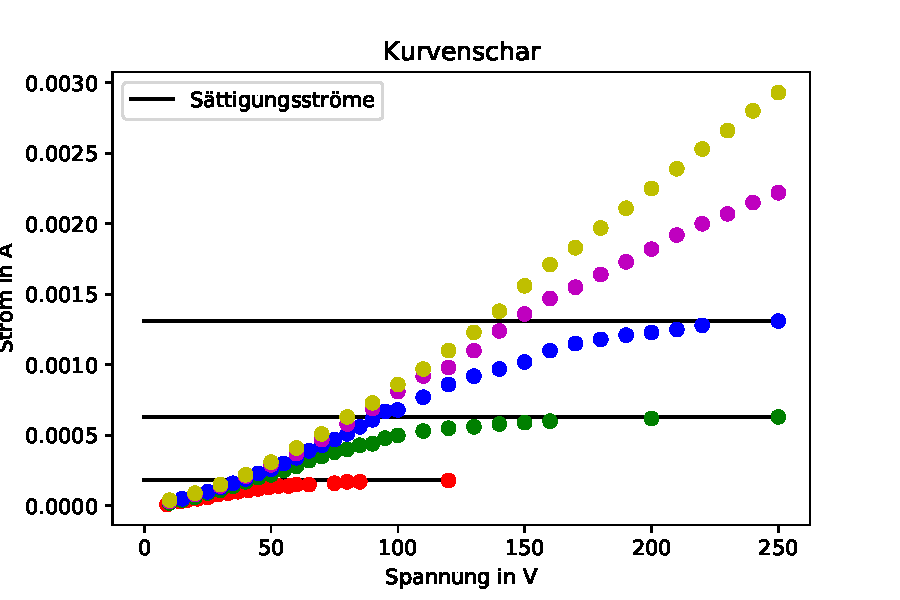
\includegraphics{schar.pdf}
    \caption{Kurvenschar der Ströme in einer Hochvakuumdiode}
    \label{fig:schar}
  \end{figure}
  
  \begin{table}
    \centering
    \caption{Sättigungsströme}
    \label{tab:vergleich}
    \sisetup{table-format=1.2}
    \begin{tabular}{S[table-format=3.2] S S S S  [table-format=3.2]}
      \toprule
      {$I_H$ in A} & {$I_s$ in A}&{$I_{s,geschätzt}$ in A}\\
      \midrule
      {$2.0$}& {$ 1.8 \times 10^{-4}$}& {$$--$$}\\
      {$2.2$}& {$ 6.3 \times 10^{-4}$}& {$$--$$}\\
      {$2.3$}& {$13.1 \times 10^{-4}$}& {$$--$$}\\
      {$2.4$}& {$\geq 22.2 \times 10^{-4}$ & {$$30.0\times 10^{-4}$$}\\
      {$2.5$}& {$\geq 29.3 \times 10^{-4}$}& {$$38.0\times 10^{-4}$$}\\
      \bottomrule
    \end{tabular}
  \end{table}
  Für die Heizströme $I_s=2.4\si[]{A}$ und $I_s=2.5\si[]{A}$ lassen sich nur untere Schranken festlegen,
  daher wurde der Wert abgeschätzt.
  

  \subsection{Bestimmung des Exponenten der Stom-Spannungs-Beziehung}
  \label{sec:exponent}
  In \autoref{fig:raumladungsgesetz} ist die Kennlinie der Diode bei dem maximal möglichen Heizstrom 
  $I_s=2.5\si[]{A}$ dargestellt und der ungefähre Gültigkeitsbereich des Langmuir-Schottkyschen-Raumladungsgesetzes, 
  zwischen Y-Achse und der eingezeichneten Linie markiert.
  \begin{figure}
    \centering
    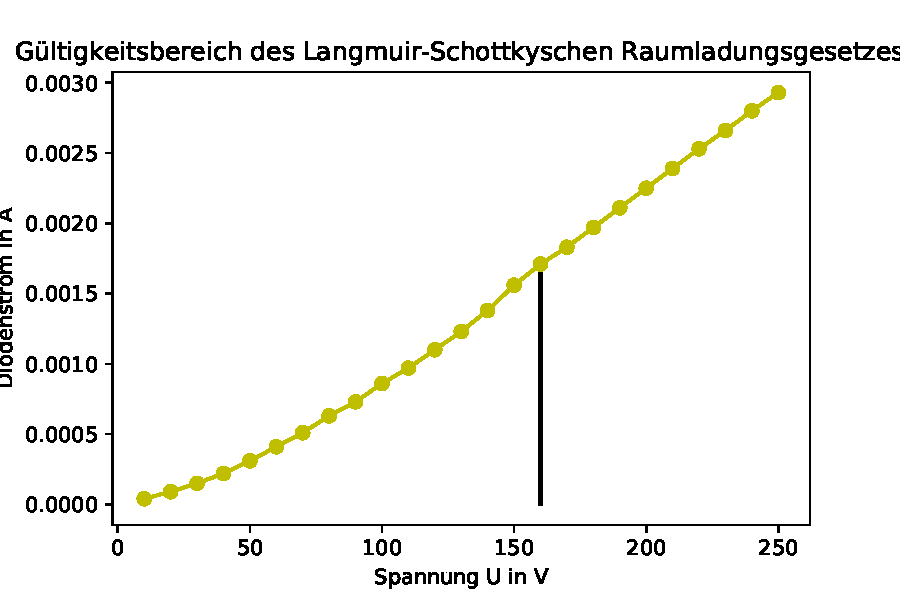
\includegraphics{raumladungsgesetz.pdf}
    \caption{Das Langmuir-Schottky-Gesetz}
    \label{fig:raumladungsgesetz}
  \end{figure}
In \autoref{fig:fit} wurde dann das Langmuir-Schottkyschen-Raumladungsgesetz an die Messwerte angepasst dafür
wurde folgende Beziehung:
\begin{center}
  $j=\frac{4}{9}\epsilon_0\sqrt{2e_0/m_0}\frac{V^{x}}{a^2}$\\
\end{center}
verwendet und durch die Python scipy Bibliothek der Divisor $a=1.475\pm 0.048$ wie auch der Exponent
$x=1.450\pm 0.014$ errechnet.
  \begin{figure}
    \centering
    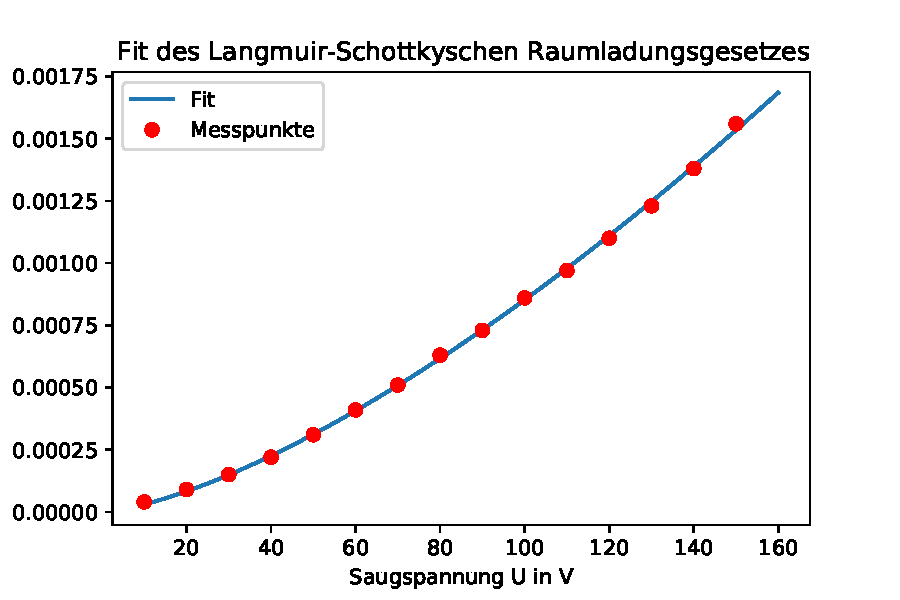
\includegraphics{fit.pdf}
    \caption{Anpassung der Strom-Spannungs-Beziehung an die Messwerte}
    \label{fig:fit}
  \end{figure}


  \subsection{Untersucheung des Anlaufstromgebietes}
  \label{sec:anlaufstromgebiet}
  Um zu untersuchen wie viele Elektronen die Anode verlassen wenn es keine Saugspannung gibt und
  welche Energie diese Elektronen haben wurde in kleinen Schritten ein Gegenfeld aufgebaut und der Kathodenstrom 
  gemessen das ergebnis ist in \autoref{fig:gegenfeld} dargestellt.

  \begin{figure}
    \centering
    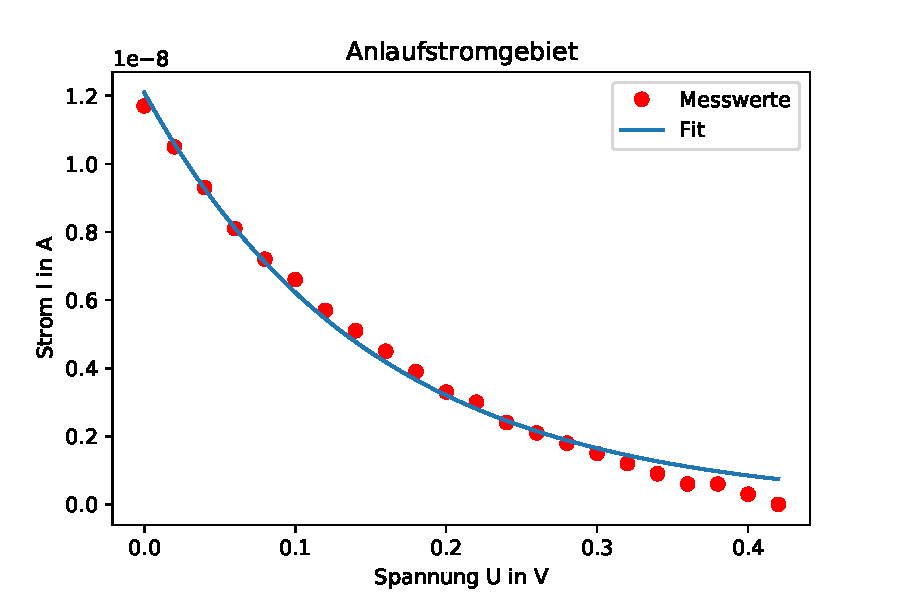
\includegraphics{anlaufstrom.pdf}
    \caption{Ströme im Gegenfeld}
    \label{fig:gegenfeld}
  \end{figure}

  An die Messwerte wurde das Gestz:
  \begin{center}
      $j(V)=const*exp(-\frac{e_0V}{kT})$
  \end{center}
  angepasst und so die Konstante $const$ und die Temperatur $T$ ermittelt. Es ergaben sich folgende Werte:
  \begin{center}
    $c=(1.20931\pm 0.2146)\times 10^{-8}$\\
    $T=1747.32\pm 48.63 \si[]{K}$
  \end{center}
  Die Anpassung an die Messwerte und die Fehlerberechnung wurden mit Hilfe der Python scypy Bibliothek erstellt.

  \subsection{Abschätzung der Kathodentemperatur}
  \label{sec:kathodentemperatur}
  Im nächste Schritt wurde dann mithilfe der Beziehung:
  \begin{center}
      $I_HU_H=f\eta \sigma T^4+N_{WL}$\\
      $\Leftrightarrow$ $T=\sqrt[4]{\frac{I_HU_H-N_{WL}}{f\eta \sigma}}$
  \end{center}
  die Kathodentemperatur bei verschiedenen Heizleistungen abgeschätzt. 
  Für $N_{WL}$ wurde der Wert $N_{WL}=0.95$ angenommen. Die Ergebnisse sind in \autoref{tab:Kathodentemperatur}
  zu sehen.

  \begin{table}
    \centering
    \caption{Kathodentemperatur}
    \label{tab:Kathodentemperatur}
    \sisetup{table-format=1.2}
    \begin{tabular}{S[table-format=3.2] S S S   [table-format=3.2]}
      \toprule
      { $I_H$ in A} & {$U_H$ in V} & {$T$ in K}\\
      \midrule
      {$$2.0$$}& {$$ 4.0 $$}&{$$1930.045$$}\\
      {$$2.2$$}& {$$ 4.0 $$}&{$$1982.611$$}\\
      {$$2.3$$}& {$$ 4.5 $$}&{$$2073.968$$}\\
      {$$2.4$$}& {$$ 5.0 $$}&{$$2159.537$$}\\
      {$$2.5$$}& {$$ 5.5 $$}&{$$2240.384$$}\\
      \bottomrule
    \end{tabular}
  \end{table}

  \subsection{Die Austrittsarbeit}
  \label{sec:arbeit}
  Um die Austrittsarbeit aus der Wolframelektrode zu berechnen wurde die Richardsongleicheung \autoref{eq:richardson}
  nach $e_0\phi$ umgestellt und für die $T$,$I_S$ wertepare berechnet. Anschießend wurde mit der Python numpy Bibliothek der
  Mittelwert und desen Feler bestimmt. Die Ergebnisse sind in \autoref{tab:austritsarbeit} dargestellt.

  \begin{table}
    \centering
    \caption{Austrittsarbeit aus einer Wolframkathode}
    \label{tab:austritsarbeit}
    \sisetup{table-format=1.2}
    \begin{tabular}{S[table-format=3.2] S S S   [table-format=3.2]}
      \toprule
      { $I_S$ in A}  & {$T$ in K}& {$e_0\phi$ in eV}\\
      \midrule
      {$$0.00018$$}& {$$1930.045$$}&{$$6.2789$$}\\
      {$$0.00063$$}& {$$1982.611$$}&{$$6.2451$$}\\
      {$$0.00131$$}& {$$2073.968$$}&{$$6.4181$$}\\
      {$$0.00222$$}& {$$2159.537$$}&{$$6.5998$$}\\
      {$$0.00293$$}& {$$2240.384$$}&{$$6.8075$$}\\
      {$$\diameter $$}& {$$--$$}&{$$6.47\pm 0.09$$}\\
      \midrule
      {$$0.0030$$}& {$$2159.537$$}&{$$6.54377$$}\\
      {$$0.0038$$}& {$$2240.384$$}&{$$6.80295$$}\\
      \bottomrule
    \end{tabular}
  \end{table}